\documentclass{beamer}
\mode<presentation>
\usepackage{amsmath}
\usepackage{amssymb}
%\usepackage{advdate}
\usepackage{adjustbox}
\usepackage{subcaption}
\usepackage{enumitem}
\usepackage{multicol}
\usepackage{mathtools}
\usepackage{listings}
\usepackage{float}
\usepackage{graphicx}
\usepackage{url}
\def\UrlBreaks{\do\/\do-}
\usetheme{Boadilla}
\usecolortheme{lily}
\setbeamertemplate{footline}
{
  \leavevmode%
  \hbox{%
  \begin{beamercolorbox}[wd=\paperwidth,ht=2.25ex,dp=1ex,right]{author in head/foot}%
    \insertframenumber{} / \inserttotalframenumber\hspace*{2ex} 
  \end{beamercolorbox}}%
  \vskip0pt%
}
\setbeamertemplate{navigation symbols}{}

\providecommand{\nCr}[2]{\,^{#1}C_{#2}} % nCr
\providecommand{\nPr}[2]{\,^{#1}P_{#2}} % nPr
\providecommand{\mbf}{\mathbf}
\providecommand{\pr}[1]{\ensuremath{\Pr\left(#1\right)}}
\providecommand{\qfunc}[1]{\ensuremath{Q\left(#1\right)}}
\providecommand{\sbrak}[1]{\ensuremath{{}\left[#1\right]}}
\providecommand{\lsbrak}[1]{\ensuremath{{}\left[#1\right.}}
\providecommand{\rsbrak}[1]{\ensuremath{{}\left.#1\right]}}
\providecommand{\brak}[1]{\ensuremath{\left(#1\right)}}
\providecommand{\lbrak}[1]{\ensuremath{\left(#1\right.}}
\providecommand{\rbrak}[1]{\ensuremath{\left.#1\right)}}
\providecommand{\cbrak}[1]{\ensuremath{\left\{#1\right\}}}
\providecommand{\lcbrak}[1]{\ensuremath{\left\{#1\right.}}
\providecommand{\rcbrak}[1]{\ensuremath{\left.#1\right\}}}
\theoremstyle{remark}
\newtheorem{rem}{Remark}
\newcommand{\sgn}{\mathop{\mathrm{sgn}}}
\providecommand{\abs}[1]{\left\vert#1\right\vert}
\providecommand{\res}[1]{\Res\displaylimits_{#1}} 
\providecommand{\norm}[1]{\lVert#1\rVert}
\providecommand{\mtx}[1]{\mathbf{#1}}
\providecommand{\mean}[1]{E\left[ #1 \right]}
\providecommand{\fourier}{\overset{\mathcal{F}}{ \rightleftharpoons}}
%\providecommand{\hilbert}{\overset{\mathcal{H}}{ \rightleftharpoons}}
\providecommand{\system}{\overset{\mathcal{H}}{ \longleftrightarrow}}
	%\newcommand{\solution}[2]{\textbf{Solution:}{#1}}
%\newcommand{\solution}{\noindent \textbf{Solution: }}
\providecommand{\dec}[2]{\ensuremath{\overset{#1}{\underset{#2}{\gtrless}}}}
\newcommand{\myvec}[1]{\ensuremath{\begin{pmatrix}#1\end{pmatrix}}}
\let\vec\mathbf

\lstset{
language=C,
frame=single, 
breaklines=true,
columns=fullflexible
}

\numberwithin{equation}{section}

\title{Presentation - Matgeo}
\author{ Sujal Chauhan\\
AI25BTECH11034 \\
EE1030 - Matrix Theory}


\begin{document}

\begin{frame}
\titlepage
\end{frame}

\section{Problem}
\begin{frame}
\frametitle{Problem Statement}
Find the distance between the points $(0,5)$ and $B(-5,0)$.
\end{frame}

\section{Solution}
\subsection{Description of Variables used}

\begin{frame}
\frametitle{Description of Variables used}
represent points as $\vec{A} $ and $\vec{B}$
\begin{table}[H]
\centering
\begin{tabular}[12pt]{ |c| c|}
    \hline
    \textbf{Input variable} & \textbf{Value}\\ 
    \hline
    $\vec{A}$ & \myvec{0 \\5 } \\
    \hline 
    $\vec{B}$ & \myvec{-5 \\ 0}\\
    \hline
    \end{tabular}
    \caption{
    \label{}
    }
 \end{table}


\end{frame}

\subsection{Theoretical Solution }
\begin{frame}
\frametitle{Theoretical Solution}
Represent the points as vectors:

\begin{align}
 \vec{A}= \myvec{0 \\ 5}, \qquad \vec{B} = \myvec{-5 \\ 0} 
\end{align}
The distance between $\vec{A}$ and $\vec{B}$ is


\begin{align}
d(\vec{A},\vec{B}) = \|\vec{B} - \vec{A}\| 
\end{align}

Subtracting the vectors,

\begin{align}
\vec{B} - \vec{A} = \myvec{0 \\ 5 } - \myvec{-5 \\ 0} = \myvec{5\\ 5}
\end{align}


Now, compute the Euclidean norm:

\begin{align}
d(\vec{A},\vec{B}) = \sqrt{(\vec{B}-\vec{A})^T(\vec{B}-\vec{A})}
\end{align}
\end{frame}

\begin{frame}
\frametitle{Theoretical Solution}

\begin{align}
d(\vec{A},\vec{B}) = \sqrt{\myvec{5& 5}\myvec{5\\ 5}} = \sqrt{50}
\end{align}


\begin{align}
 d(\vec{A},\vec{B}) = 5\sqrt{2}
\end{align}



\textbf{Final Answer:}

\begin{align}
 d(\vec{A},\vec{B}) = \|\vec{B} - \vec{A}\| = 5\sqrt{2}
\end{align}



\end{frame}

\subsection{Plot}
\begin{frame}
    \frametitle{Plot}
\begin{figure}[H]
   \centering
   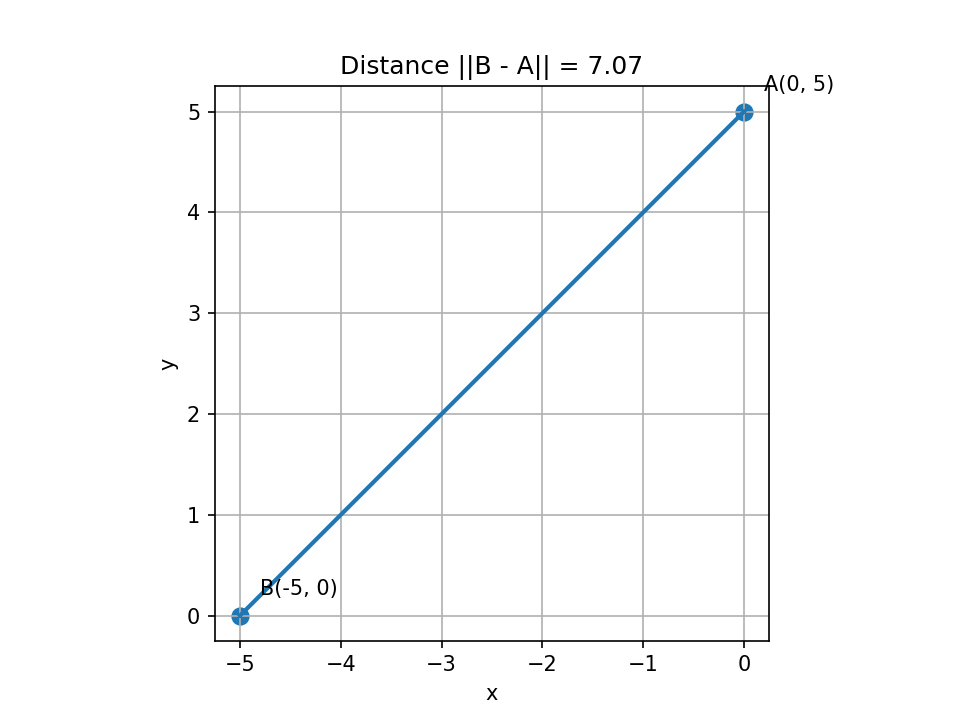
\includegraphics[width=0.9\columnwidth]{figures/distance.png}
   \end{figure}
\end{frame}







\end{document}